% !Mode:: "TeX:UTF-8"
% !TEX program  = xelatex

%\documentclass{cumcmthesis}
\documentclass[withoutpre]{cumcmthesis} %去掉封面与编号页
\usepackage[framemethod=TikZ]{mdframed}
\usepackage{url}   % 网页链接
\usepackage{subcaption} % 子标题
\title{穿越沙漠}
\tihao{A}
\baominghao{202010038016}
\schoolname{南京大学}
\membera{陈万驰 181840033 数学系}
\memberb{姜玉骅 181870080 工程管理学院}
\memberc{佘帅杰 181860077 计算机科学与技术系}
\supervisor{教练组}
\yearinput{2020}
\monthinput{08}
\dayinput{1}

\begin{document}

 \maketitle
 \begin{abstract}


\keywords{新冠肺炎疫情 \quad SEIR 模型 \quad 混样检测}
\end{abstract}

%目录  2019 明确不要目录,我觉得这个规定太好了
%\tableofcontents

%\newpage

\section{问题重述}
考虑如下的小游戏:玩家凭借一张地图,利用初始资金购买一定数量的水和食物(包括食品和其他日常用品),从起点出发,在沙漠中行走。途中会遇到不同的天气,也可在矿山、村庄补充资金或资源,目标是在规定时间内到达终点,并保留尽可能多的资金。
游戏的基本规则如下:
\begin{enumerate}
    \item 以天为基本时间单位,游戏的开始时间为第0天,玩家位于起点。玩家必须在截止日期或之前到达终点,到达终点后该玩家的游戏结束。
    \item 穿越沙漠需水和食物两种资源,它们的最小计量单位均为箱。每天玩家拥有的水和食物质量之和不能超过负重上限。若未到达终点而水或食物已耗尽,视为游戏失败。
    \item 每天的天气为“晴朗”、“高温”、“沙暴”三种状况之一,沙漠中所有区域的天气相同。
    \item 每天玩家可从地图中的某个区域到达与之相邻的另一个区域,也可在原地停留。沙暴日必须在原地停留。
    \item 玩家在原地停留一天消耗的资源数量称为基础消耗量,行走一天消耗的资源数量为基础消耗量的2倍。
    \item 玩家第0天可在起点处用初始资金以基准价格购买水和食物。玩家可在起点停留或回到起点,但不能多次在起点购买资源。玩家到达终点后可退回剩余的水和食物,每箱退回价格为基准价格的一半。
    \item 玩家在矿山停留时,可通过挖矿获得资金,挖矿一天获得的资金量称为基础收益。如果挖矿,消耗的资源数量为基础消耗量的 倍;如果不挖矿,消耗的资源数量为基础消耗量。到达矿山当天不能挖矿。沙暴日也可挖矿。
    \item 玩家经过或在村庄停留时可用剩余的初始资金或挖矿获得的资金随时购买水和食物,每箱价格为基准价格的2倍。
\end{enumerate}
    需要解决以下三个问题。
\begin{enumerate}
    \item 假设只有一名玩家,在整个游戏时段内每天天气状况事先全部已知,试给出一般情况下玩家的最优策略。求解附件中的“第一关”和“第二关”,并将相应结果分别填入Result.xlsx。
    \item 假设只有一名玩家,玩家仅知道当天的天气状况,可据此决定当天的行动方案,试给出一般情况下玩家的最佳策略,并对附件中的“第三关”和“第四关”进行具体讨论。
    \item 现有$n$名玩家,他们有相同的初始资金,且同时从起点出发。若某天其中的任意$k$名玩家均从区域$A$行走到区域$B$,则他们中的任一位消耗的资源数量均为基础消耗量的$2k$倍;若某天其中的任意 $k$玩家在同一矿山挖矿,则他们中的任一位消耗的资源数量均为基础消耗量的3倍,且每名玩家一天可通过挖矿获得的资金是基础收益的 ;若某天其中的任意 名玩家在同一村庄购买资源,每箱价格均为基准价格的$\frac{1}{k}$倍。其他情况下消耗资源数量与资源价格与单人游戏相同。
    \begin{enumerate}
        \item 假设在整个游戏时段内每天天气状况事先全部已知,每名玩家的行动方案需在第1天确定且此后不能更改。试给出一般情况下玩家应采取的策略,并对附件中的“第五关”进行具体讨论。
        \item 假设所有玩家仅知道当天的天气状况,从第2天起,每名玩家在当天行动结束后均知道其余玩家当天的行动方案和剩余的资源数量,随后确定各自第二天的行动方案。试给出一般情况下玩家应采取的策略,并对附件中的“第六关”进行具体讨论。
    \end{enumerate}

\end{enumerate}


\section{问题分析}
\subsection{问题一分析}


\subsection{问题二分析}


\subsection{问题三分析}


\subsection{问题四分析}


混样检测,顾名思义就是将几个样本混合在一起进行一次核酸检测。某次需要对$N$个人进行检测,病毒的携带率为$p$。为了减少工作量,一次性将$k$个人的样本混合,如果混合样本为阴性,则说明这$k$个人都没有患病。如果混合样本为阳性,说明这$k$个人中至少有1个人的样本是阳性,那么接下来对这$k$个人的分别单独做检测。而单次检测简单直观,即对所有人单独做检测。考虑用基本概率论知识,比较混样检测和单次检测方法对应到平均每人的检测次数,选取更合理的方案。

\section{模型假设}
\begin{enumerate}
    \item 假设人群中所有个体都有被感染的概率。
    \item 假设被感染个体痊愈后,会产生抗体,不会再被感染。
    \item 假设所有感染者是同质的,即病情的严重程度、死亡率相同。
    \item 鉴于1月23日武汉市封城,假设武汉市总人口的不变。
    \item 假设核酸检测准确率为100\%。
    \item 假设混样检测的结果不会因混样而改变,即若至少有一人感染,混样检测呈阳性;若无人感染,混样检测呈阴性。
\end{enumerate}

\section{符号说明}
\begin{table}[H]
    \caption{符号说明表}\label{tab:001} \centering
    \begin{tabular}{ccc}
        \toprule[1.5pt]
        \textbf{参数} & \textbf{定义} & \textbf{单位}\\
        \midrule[1pt]
        $W$ & 负重上限 & 千克\\ 
        $M$ & 初始资金 & 元 \\
        $t$ & 天数 & 天\\
        $T$ & 总天数 & 天\\
        $m_w$ & 每箱水的质量 & 千克/箱\\
        $m_f$ & 每箱食物的质量 & 千克/箱 \\
        $p_w$ & 水的基准价格 & 元/箱\\
        $p_f$ & 食物的基准价格 & 元/箱\\
        $n_{sw}$ & 晴朗天气下水的基准消耗量 & 箱\\
        $n_{hw}$ & 高温天气下水的基准消耗量 & 箱\\
        $n_{ow}$ & 沙暴天气下水的基准消耗量 & 箱\\
        $n_{sf}$ & 晴朗天气下食物的基准消耗量 & 箱\\
        $n_{hf}$ & 高温天气下食物的基准消耗量 & 箱\\
        $n_{of}$ & 沙暴天气下食物的基准消耗量 & 箱\\
        $n$ & 玩家数 & 人 \\
        $P_{t}$ & 第t天开始时玩家所处的位置 & / \\
        $W_{t}$ & 第t天开始时玩家剩余的水 & 箱 \\
        $F_{t}$ & 第t天开始时玩家剩余的食物 & 箱 \\ 
        $Q_{t}$ & 第t天开始时玩家剩余的资金 & 元 \\
        $S_{t}$ & 第t天玩家所处的地点特征 & /\\
        $Wea_t$ & 第t天的天气 & /\\
        $Q_{Mine}$ & 基础收益 & 元\\
        
        \bottomrule[1.5pt]
    \end{tabular}
\end{table}


\section{模型建立与求解}
\subsection{游戏模型的建立}

我们首先将该游戏利用数学语言加以描述。显然该局游戏的最终目的是使玩家到达终点时的收益最大,即\\\\
\begin{equation}
	\max Q_{30}+\frac{1}{2}p_wW_{30}+\frac{1}{2}p_fF_{30}
\end{equation}
其中$Q_{t},W_{t},F_{t}$分别表示第t天时玩家所剩下的资金、水和食物量。如果玩家在第30天前到达终点,则其各个属性将会在未来几天视作不变,所以我们以第三十天为统一结束时间。该目标函数有如下约束:\\\\
\begin{equation}
	Q_t=Q_{t-1}+Q_{Mine}Mine_t-Shop_t[2p_fShopF_t+2p_wShopW_t]
\end{equation}
其中$$Mine_t=\begin{cases}
0,\quad \text{如果第t天不挖矿}\\
1,\quad \text{如果第t天挖矿}
\end{cases}$$
$$Shop_t=\begin{cases}
0,\quad \text{如果第t天不购物}\\
1,\quad \text{如果第t天购物}
\end{cases}$$
即每天结束时的资金等于前一天的资金加上当天挖矿获得的1000元(如果挖矿的话),再减去在村庄购买食物和水花费的钱(如果购买的话)。其中$ShopF_t$和$ShopW_t$分别表示玩家在第t天购买的食物量和水量(如果购买的话)。\\\\
\begin{equation}
F_t=F_{t-1}-2Move_t\triangle F_t-3Mine_tMove_t\triangle F_t-(1-Move_t-Mine_t)\triangle F_t+Shop_tShopF_t
\end{equation}
即每天结束时的食物量等于前一天的食物量减去当天的食物消耗量再加上在村庄购买的食物量(如果购买的话)。\\\\
\begin{equation}
W_t=W_{t-1}-2Move_t\triangle W_t-3Mine_t\triangle W_t-(1-Move_t-Mine_t)\triangle W_t+Shop_tShopW_t
\end{equation}
即每天结束时的水量等于前一天的水量减去当天的水消耗量再加上在村庄购买的水量(如果购买的话)。\\\\
\begin{equation}
P_{t}=P_{t-1}(1-Move_t)+\bar{P}_{t-1}Move_t
\end{equation}
其中$P_t$表示第t天的位置,$\bar{P_t}$表示第t+1天可以到达的几个相邻区域之一,
$$Move_t=\begin{cases}
1,\quad \text{如果第t天移动}\\
0,\quad \text{如果第t天不移动(包括挖矿、停留)}
\end{cases}$$\\\\
\begin{equation}
Shop_t\leqslant If_0[(P_t-C_1)(P_t-C_2)\cdots(P_t-C_n)]
\end{equation}
\begin{equation}
Mine_t\leqslant If_0[(P_{t-1}-K_1)(P_{t-1}-K_2)\cdots(P_{t-1}-K_m)]
\end{equation}其中$C_1,C_2,\cdots,C_n$表示n个村庄的位置,$K_1,K_2,\cdots,K_m$表示m个矿山的位置,
$$If_0(x)=\begin{cases}
1,\quad if\quad x=0\\\\
0,\quad if\quad x\neq0
\end{cases}$$\\\\

$\triangle F$和$\triangle W$分别表示第t天基础消耗的食物量和水量,由Lagrange插值公式:
$$L(x)=\sum_{i=1}^nf(x_i)\displaystyle\frac{\Pi_{j\neq i}(x-x_j)}{\Pi_{j\neq i}(x_i-x_j)}$$
可得
\begin{equation}
\triangle F_t=n_{sf}\frac{Wea_t^2-3Wea_t+2}{2}+n_{hf}\frac{Wea_t^2-2Wea_t}{-1}+n_{of}\frac{Wea_t^2-Wea_t}{2}
\end{equation}
\begin{equation}
\triangle W_t=n_{sw}\frac{Wea_t^2-3Wea_t+2}{2}+n_{hw}\frac{Wea_t^2-2Wea_t}{-1}+n_{ow}\frac{Wea_t^2-Wea_t}{2}
\end{equation}
其中$$Wea_t=\begin{cases}
0,\quad\text{晴朗天气}\\
1,\quad\text{高温天气}\\
2,\quad\text{沙暴天气}
\end{cases}$$表示第t天的天气情况。



\subsection{地图简化}

我们首先引入Dijkstra算法,这是一种在有向赋权图中求两点之间最短路径的高效算法。
\begin{figure}[H]
	\centering
	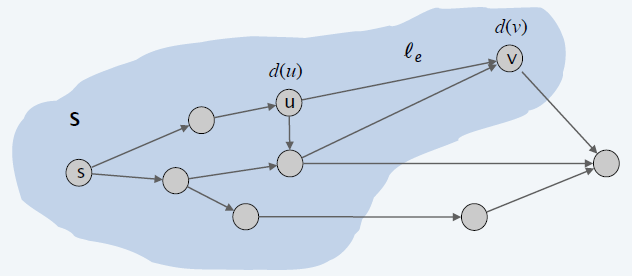
\includegraphics[scale=0.7]{figures/Dijkstra.png}
	\caption{Dijkstra算法示意图}
	\label{fig:Dijkstra}
\end{figure}
如图\ref{fig:Dijkstra},该图中s是起点,最右侧的点是终点。$d(u)$表示从点$s$到点$u$的最短距离。之后执行如下操作:\\
(1)初始化$S={s},d(s)=0$;\\
(2)反复寻找未探索过的点v,使得$\min\quad\pi(v)$,将$v$添加到$S$中,并且$d(v)=\pi(v)$,其中
$$\pi(v)=\min_{e=(u,v):u\in S}d(u)+distance(arg\min_{e=(u,v):u\in S}d(u),v)$$
最终当终点属于$S$时,可以知道起点到终点的最短路径长度,从而问题求解。\\\\
可以看出,问题一的核心关键在于玩家是否前往矿山挖矿、在矿山连续挖几天矿、在挖矿之后是否需要前往村庄补给物资以及是否可以在矿山和村庄之间往返。我们将问题作如下简化:

选取图中起点、终点、村庄和矿山作为特殊点,利用Dijkstra算法计算出每两个特殊点之间的最短路径(即不考虑沙暴天气的影响下,所需最少的天数),如图\ref{fig:map1}:
\begin{figure}[H]
	\centering
	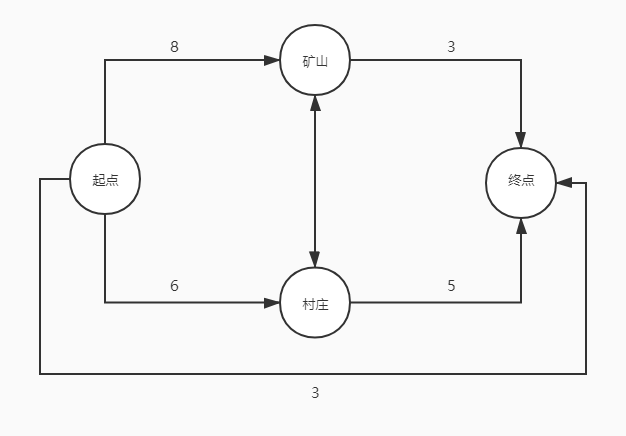
\includegraphics[scale=0.5]{figures/map1new.jpg}
	\caption{简化后的Map1}
	\label{fig:map1}
\end{figure}
该图是一个完全图(即图中每两点之间都有一条边),且每条边上的数字代表着两个特殊点之间的最短路径(受天气影响可能会有变化)。其中:$P_0$代表起点,$P_1$代表村庄,$P_2$代表矿山,$P_3$代表终点。对于问题一,因为天气是预先给定的,整局游戏没有随机因素,所以我们假定玩家在游戏途中始终向着某个特殊点(终点、村庄、矿山)前进并且选择最合适的路径,而非漫无目的地随机移动,即游戏旅程由几条有向线段叠加而成:
\begin{equation}
	\overrightarrow{P}=\sum_{k=1}^{n}\overrightarrow{P_{i_k}P_{i_{k+1}}}
\end{equation}
其中$i_k\leqslant3,\quad k=1,2,\dots,n$.

\subsection{路径方案}
%参考文献
\begin{thebibliography}{9}%宽度9

    

\end{thebibliography}

\end{document} 